% 06_training.tex — Capitolo 6: Come impara una rete: training e backpropagation.
% Documento didattico "Intelligenza artificiale nel progetto supervised_telemedicina".

\chapter{Come impara una rete: training e backpropagation}\label{cap:training}

Nel capitolo~\ref{cap:reti} abbiamo visto la struttura del MLP di
\progetto{}: una funzione parametrica che mappa 6 feature in 3 probabilità.
Ma una rete non si programma: si \emph{addestra}. In questo capitolo vediamo
come, partendo da una funzione di perdita, si arriva all'aggiornamento dei
pesi con la discesa del gradiente e la backpropagation, e come il progetto
\progetto{} organizza il training nel file
\file{training/train\_model.py}.

\section{La funzione di perdita}\label{sec:funzione-perdita}

Per addestrare una rete serve un modo per misurare \emph{quanto è sbagliata}
la previsione. La funzione di perdita (o loss) assegna un numero a ogni
previsione: più è alto, più il modello è lontano dalla verità. Il progetto
usa la \emph{cross-entropy}:

\begin{equation}
L = -\frac{1}{N} \sum_{i=1}^{N} \log p_{y_i},
\end{equation}

dove $p_{y_i}$ è la probabilità che il modello assegna alla classe corretta
$y_i$ per il campione $i$-esimo. Perché il logaritmo? Perché la probabilità
della classe corretta è un numero tra 0 e 1: il suo logaritmo è negativo e
tanto più grande in valore assoluto quanto più la probabilità è piccola.
Se il modello è sicuro e azzecca ($p_{y_i} \approx 1$), il contributo è
$\approx 0$; se sbaglia con sicurezza ($p_{y_i} \approx 0$), il contributo
esplode. È l'equivalente di un \codice{log} in un sistema di logging: gli
errori rari ma gravi pesano molto di più.

Nel codice (\file{src/telemedicina\_supervised/ml/mlp.py}) la loss è
implementata con un clip anti \codice{log(0)}:

\begin{lstlisting}[caption={Cross-entropy media in \file{mlp.py} (metodo \codice{loss}).}]
def loss(self, X: np.ndarray, y: np.ndarray) -> float:
    """Cross-entropy media; clip anti log(0)."""
    probs = self.probabilità(X)
    n = probs.shape[0]
    probs_scelte = np.clip(probs[np.arange(n), y], _EPS_LOG, 1.0)
    return float(-np.mean(np.log(probs_scelte)))
\end{lstlisting}

La riga \codice{probs[np.arange(n), y]} seleziona, per ogni campione, la
probabilità della classe corretta: è l'indicizzazione vettoriale di numpy
che fa in una riga quello che in un linguaggio imperativo richiederebbe un
ciclo.

\section{La discesa del gradiente}\label{sec:discesa-gradiente}

La loss è una funzione di tutti i parametri $\theta = (W_1, b_1, W_2, b_2)$.
Vogliamo trovare i parametri che la minimizzano. Il gradiente
$\nabla_\theta L$ è il vettore delle derivate parziali: indica la direzione
di \emph{maggiore crescita} della loss. Per minimizzare, ci muoviamo nella
direzione opposta:

\begin{equation}
\theta \leftarrow \theta - \eta \nabla_\theta L,
\end{equation}

dove $\eta$ (il \emph{learning rate}) è la dimensione del passo.

L'analogia classica è scendere una collina nella nebbia: non vedi la valle,
ma senti la pendenza sotto i piedi e fai un passo nella direzione in cui il
terreno scende di più. Il learning rate è la lunghezza del passo:

\begin{itemize}
  \item troppo \emph{alto}: si rischia di saltare oltre il minimo e
        oscillare o divergere (come fare passi troppo lunghi su una collina
        ripida);
  \item troppo \emph{basso}: si scende lentissimamente e si rischia di
        fermarsi molto prima del minimo (come avanzare di un millimetro alla
        volta).
\end{itemize}

Nel progetto il learning rate è uno degli iperparametri della griglia di
ricerca (sezione~\ref{sec:ricerca-griglia}): i valori provati sono
\codice{0.01} e \codice{0.05}.

\section{La backpropagation}\label{sec:backpropagation}

Per applicare la discesa del gradiente serve calcolare
$\nabla_\theta L$: le derivate della loss rispetto a ogni peso. La
\emph{backpropagation} è l'algoritmo che lo fa in modo efficiente,
applicando la \emph{regola della catena} del calcolo differenziale: la
derivata di una funzione composta è il prodotto delle derivate dei singoli
passi.

Nel nostro MLP la catena è: $x \to z_1 \to a_1 \to z_2 \to p \to L$. Il
gradiente si propaga \emph{all'indietro}: prima $\partial L / \partial z_2$
(dalla softmax e dalla cross-entropy), poi attraverso la ReLU fino a
$\partial L / \partial z_1$, e infine ai pesi. Il codice reale in
\file{src/telemedicina\_supervised/ml/mlp.py} (metodo \codice{gradienti})
è il seguente:

\begin{lstlisting}[caption={Backpropagation in \file{mlp.py} (metodo \codice{gradienti}).}]
def gradienti(self, X: np.ndarray, y: np.ndarray) -> Dict[str, np.ndarray]:
    avanti = self.forward(X)
    probs, a1, z1 = avanti["probs"], avanti["a1"], avanti["z1"]
    n = X.shape[0]

    # dL/dz2 per softmax + cross-entropy: (probs - onehot) / n.
    onehot = np.zeros_like(probs)
    onehot[np.arange(n), y] = 1.0
    dz2 = (probs - onehot) / n

    dW2 = dz2.T @ a1
    db2 = np.sum(dz2, axis=0)

    # Chain rule attraverso ReLU (derivata 1 dove z1 > 0).
    da1 = dz2 @ self.W2
    dz1 = da1 * (z1 > 0)

    dW1 = dz1.T @ X
    db1 = np.sum(dz1, axis=0)

    return {"W1": dW1, "b1": db1, "W2": dW2, "b2": db2}
\end{lstlisting}

Nota la riga \codice{dz1 = da1 * (z1 > 0)}: la derivata della ReLU è 1 dove
$z_1 > 0$ e 0 altrove, quindi il gradiente ``passa'' solo attraverso i
neuroni attivi. È l'equivalente di un \codice{mask} in numpy.

\begin{esempio}{La regola della catena in pratica}
La derivata della loss rispetto a $W_2$ si ottiene moltiplicando la
derivata rispetto a $z_2$ per la derivata di $z_2$ rispetto a $W_2$:
$\partial L / \partial W_2 = (\partial L / \partial z_2) \cdot a_1$.
Nel codice: \codice{dW2 = dz2.T @ a1}. Ogni riga del metodo
\codice{gradienti} corrisponde a un anello della catena.
\end{esempio}

\section{Il ciclo di training}\label{sec:ciclo-training}

Il training procede per \emph{epoche}: ogni epoca è una passata completa sul
dataset di training, diviso in \emph{mini-batch}. Per ogni batch si calcola
il gradiente e si aggiornano i pesi. Prima di ogni epoca i campioni vengono
\emph{mescolati} (\codice{rng.permutation(n)}): l'ordine dei batch cambia a
ogni epoca, il che rende l'ottimizzazione più stabile. Il codice reale del
ciclo (metodo \codice{train} in \file{src/telemedicina\_supervised/ml/mlp.py},
abbreviato) è:

\begin{lstlisting}[caption={Ciclo di training in \file{mlp.py} (metodo \codice{train}, abbreviato).}]
for epoca in range(epoche):
    ordine = rng.permutation(n)
    for inizio in range(0, n, batch_size):
        indice = ordine[inizio : inizio + batch_size]
        X_b, y_b = X[indice], y[indice]
        gradi = self.gradienti(X_b, y_b)
        self._aggiorna(gradi, lr)

    loss_tr = self.loss(X, y)
    storia["loss_train"].append(loss_tr)
    if X_val is not None and y_val is not None:
        loss_va = self.loss(X_val, y_val)
    else:
        loss_va = loss_tr
    storia["loss_val"].append(loss_va)

    if loss_va < migliore_loss:
        migliore_loss = loss_va
        migliore_pesi = self._pesi()
        epoche_senza_miglioramento = 0
    else:
        epoche_senza_miglioramento += 1
        if epoche_senza_miglioramento >= pazienza:
            break
\end{lstlisting}

L'aggiornamento dei pesi è la discesa del gradiente in forma vettoriale:

\begin{lstlisting}[caption={Aggiornamento dei pesi (metodo \codice{\_aggiorna}).}]
def _aggiorna(self, gradi: Dict[str, np.ndarray], lr: float) -> None:
    self.W1 -= lr * gradi["W1"]
    self.b1 -= lr * gradi["b1"]
    self.W2 -= lr * gradi["W2"]
    self.b2 -= lr * gradi["b2"]
\end{lstlisting}

Ogni riga è esattamente $\theta \leftarrow \theta - \eta \nabla_\theta L$
applicata a una matrice di parametri.

\section{Early stopping}\label{sec:early-stopping}

Il ciclo di training ha un meccanismo di arresto anticipato: se la loss di
\emph{validazione} non migliora per \codice{pazienza} epoche consecutive
(nel progetto \codice{PAZIENZA = 5}, vedi
\file{src/telemedicina\_supervised/config.py}), il training si ferma e
vengono ripristinati i pesi migliori. Perché? Perché la loss di training
può continuare a scendere anche quando il modello ha smesso di generalizzare
e sta semplicemente \emph{memorizzando} i dati di training: è l'
\emph{overfitting}. La loss di validazione è il campanello d'allarme: se
sale mentre quella di training scende, il modello sta imparando a memoria.

La figura~\ref{fig:loss-curve} mostra le curve di loss del training finale
del progetto. La linea tratteggiata rossa segna l'epoca della migliore loss
di validazione (epoca 24, loss $\approx 0.051$): è il punto in cui il
modello generalizza meglio, e il punto che l'early stopping ripristina a
fine training.

\begin{figure}[htbp]
  \centering
  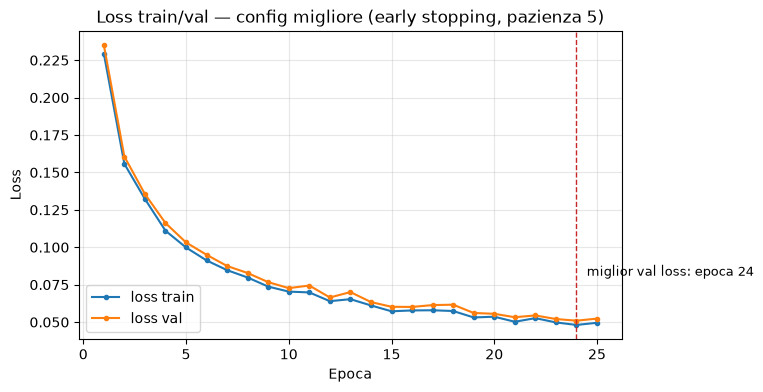
\includegraphics[width=0.85\textwidth]{figure/generate/loss_curve.png}
  \caption{Loss di training e validazione per la configurazione migliore
  (25 epoche). La linea tratteggiata rossa indica l'epoca della migliore
  loss di validazione: con pazienza 5, il training si sarebbe fermato dopo
  5 epoche consecutive senza miglioramento.}
  \label{fig:loss-curve}
\end{figure}

\section{La ricerca a griglia}\label{sec:ricerca-griglia}

Il progetto non addestra un solo modello: confronta sei configurazioni di
iperparametri definite in \file{src/telemedicina\_supervised/config.py}
(la griglia \codice{GRID}), tutte con 25 epoche e pazienza 5. La
tabella~\ref{tab:griglia} le riassume.

\begin{table}[htbp]
  \centering
  \caption{Le sei configurazioni della griglia di \file{config.py}. La
  selezione avviene sulla loss di validazione minima; il report del progetto
  (\file{data/models/report.json}) registra come vincitrice la
  configurazione con $n = 32$, \codice{lr} = 0.05, batch 32, con loss di
  validazione $\approx 0.051$.}
  \label{tab:griglia}
  \begin{tabular}{cccc l}
    \toprule
    \codice{n\_hidden} & \codice{lr} & \codice{batch\_size} & \codice{epoche} & esito \\
    \midrule
    16 & 0.01 & 32 & 25 & non selezionata \\
    16 & 0.05 & 32 & 25 & non selezionata \\
    32 & 0.01 & 32 & 25 & non selezionata \\
    32 & 0.05 & 32 & 25 & selezionata \\
    64 & 0.01 & 64 & 25 & non selezionata \\
    64 & 0.05 & 64 & 25 & non selezionata \\
    \bottomrule
  \end{tabular}
\end{table}

La funzione \codice{seleziona\_migliore} in
\file{training/train\_model.py} addestra ogni configurazione e tiene quella
con la loss di validazione minima:

\begin{lstlisting}[caption={Selezione della configurazione migliore in \file{train\_model.py} (abbreviato).}]
for config in GRID:
    modello, storia = addestra_configurazione(
        X_train, y_train, X_val, y_val, config, seed
    )
    loss_val = min(storia["loss_val"])
    if loss_val < migliore_loss:
        migliore_loss = loss_val
        migliore_config = config
\end{lstlisting}

Nota un dettaglio metodologico importante: la scelta avviene sulla
\emph{validazione}, mai sul test. Il test congelato viene usato una sola
volta, alla fine, per la valutazione finale
(capitolo~\ref{cap:valutazione}). Usare il test per scegliere gli
iperparametri sarebbe un \emph{leakage}: i numeri finali sarebbero
ottimistici \cite{progetto2026}.

\section{Il gradient check}\label{sec:gradient-check}

La backpropagation è un algoritmo delicato: un errore di segno o di indice
in una derivata produce gradienti sbagliati che il training non può
rilevare da solo. Per questo il progetto include una \emph{verifica
numerica} in \file{src/telemedicina\_supervised/ml/gradient\_check.py}: i
gradienti analitici vengono confrontati con quelli calcolati per
\emph{differenze finite centrali},

\begin{equation}
\frac{\partial L}{\partial \theta_i} \approx
\frac{L(\theta_i + \varepsilon) - L(\theta_i - \varepsilon)}{2\varepsilon},
\end{equation}

con $\varepsilon = 10^{-6}$. Se la backpropagation è corretta, i due
gradienti coincidono quasi esattamente: nel progetto l'errore relativo
massimo è dell'ordine di $10^{-10}$, ben al di sotto della soglia di
accettazione del test (\codice{< 2e-5} in \file{tests/test\_mlp.py}). È la
prova che la regola della catena è stata implementata correttamente, come
sottolinea anche Bishop nel suo trattamento della backpropagation
\cite{bishop2006pattern}.

\begin{esempio}{Il gradient check in \progetto{}}
La funzione \codice{errore\_massimo\_relativo} in
\file{gradient\_check.py} calcola, per ogni parametro, l'errore relativo
$\lvert a - n \rvert / \max(1, \lvert a \rvert, \lvert n \rvert)$ tra
gradiente analitico ($a$) e numerico ($n$), e restituisce il massimo su
tutti i parametri. Un valore sotto $\sim 10^{-5}$ indica un backward
corretto.
\end{esempio}